\chapter{Neutral Current Event Selection}
\label{ch:Selection}

The NC disappearance analysis is performed by comparing the observed FD spectrum of NC events to the predicted number of events after extrapolation. This requires a largely pure sample of NC signal events. There are three main backgrounds for this sample, $\nue$ CC interactions, $\numu$ CC interactions, and cosmic ray events. This chapter describes the full process for selecting a sample of NC events and eliminating backgrounds, briefly discussing data quality and event quality metrics, and fully detailing the fiducial, containment, NC selection, and cosmic rejection.

The analysis specific cuts were chosen based on the official second analysis (SA) files. These files were produced in tag \verb|R16-03-03|, and NuS group specific DeCAF files were produced in tag \verb|S16-04-08|. These files included MEC events, and the corresponding Tufts CC weight was applied to all (applicable) events \cite{ref:TNGENIE}. For normalization simplicity, only $14$ diblock MC and data were studied. After applying this criterion, all beam spectra were scaled to \pot{6}, and the cosmic spectra were scaled to $120\unit{s}$. The cuts were set assuming the $3$ flavor oscillation parameters listed in table \ref{tab:3FlavParams}. The remainder of this chapter describes each level of event cut and their affect on the ND and FD spectra.
\begin{table}[htb]
  \begin{center}
    \begin{tabular}{c c}
      \hline\hline
      Oscillation Parameter & Value \\
      \hline
      $\rho$ & $2.84\unit{g/cm\textsuperscript{3}}$ \\
      $\Delta m^2_{21}$ & $7.53 \times 10^{-5}\evsq$ \\
      $\sin^2 2\theta_{12}$ & $0.846$ \\
      $\Delta m^2_{32}$ & $2.37 \times 10^{-3}\evsq$ \\
      $\theta_{23}$ & $\pi/4$ \\
      $\sin^2 2\theta_{13}$ & $0.085$ \\
      $\delta$ & $0$ \\
      \hline
    \end{tabular}
    \caption[Assumed Oscillation Parameters]{The $3$ flavor oscillation parameters assumed for studying the NC selection cuts}
    \label{tab:3FlavParams}
  \end{center}
\end{table}

\section{A Note on Preselection}
\label{sec:SelVeto}

The cuts discussed in this chapter were trained on cosmic trigger data files. These files had a cosmic veto motivated by the $\nue$ appearance analysis baked directly into the files. The cuts used are described in reference \cite{ref:CosmicVetoNue}. The actual cosmic prediction will came from the NuMI out of time side band which will had a more generalized cosmic veto. 

\section{Data Quality}
\label{sec:SelDQ}

Data quality cuts were developed well before the first \nova~results to ensure proper data taking conditions, and all analysis groups apply them as standard. These cuts are applied per spill, and spills that fail these cuts are not included in POT accounting. The cuts can be categorized into three main groups, beam quality, data quality, and timing. The beam quality cuts were studied and set as described in reference \cite{ref:TNBeamQual}. To be included, spills must meet all of the criteria listed in table \ref{tab:BeamQual}. Two event quality cuts were applied to data from each detector. These cuts were motivated and set as described in references \cite{ref:DQND, ref:DQFDDCMLiveGeo, ref:DQFDDCMEdgeFrac}, and are summarized in table \ref{tab:DataQual}. Finally, a timing cut is applied to cosmic data to ensure that the data is not too close to the edge of the data taking window. For cosmic events within a given $500\,\mu s$ trigger window, only events between $25\,\mu{\mbox{s}} < t < 475\,\mu{\mbox{s}}$ are kept. Table \ref{tab:NP1DataQual} shows the number of events that pass these data quality cuts, and figure \ref{fig:NP1DataQual} shows the energy spectra at the ND and FD.
\begin{table}[htb]
  \begin{center}
    \begin{tabular}{c c c}
      \hline\hline
      Beam Quality Parameter & Minimum & Maximum \\
      \hline
      Spill POT & $2.00 \times 10^{12}$ & \\
      Horn Current & $-202\unit{kA}$ & $-198\unit{kA}$ \\
      Beam X and Y position on target & $0.02\unit{mm}$ & $2.00\unit{mm}$ \\
      Beam X and Y width & $0.57\unit{mm}$ & $1.58\unit{mm}$ \\
      Time to nearest beam spill & & $0.5\unit{s}$ \\
      \hline
    \end{tabular}
    \caption[Beam Quality Cuts]{Beam quality cuts applied to each spill to ensure proper data taking conditions. Taken from reference \cite{ref:TNBeamQual}.}
    \label{tab:BeamQual}
  \end{center}
\end{table}

\begin{table}[htb]
  \begin{center}
    \begin{tabular}{c c c}
      \hline\hline
      Data Quality Parameter & Detector & Metric for Spill to Pass \\
      \hline
      Number of Missing DCMs & ND & $= 0$ \\
      Lights On Effect Hit Fraction & ND & $\leq 0.45$ \\
      Missing DCMs from LiveGeometry & FD & $= 0$ \\
      DCM Edge Match Fraction & FD & $> 0.2$ \\
      \hline
    \end{tabular}
    \caption[Data Quality Cuts]{Data quality cuts applied to each spill to ensure proper data taking conditions.}
    \label{tab:DataQual}
  \end{center}
\end{table}

\begin{table}[htb]
  \begin{center}
    \begin{tabular}{c c c c c}
      \hline\hline
      Cut Level & NC & $\numu$ CC & $\nue$ CC & Cosmic \\
      \hline
      \multicolumn{5}{l}{FD:} \\
      Data Quality & $337.0$ & $230.6$ & $58.5$ & $23.4 \times 10^{6}$ \\
      \multicolumn{5}{l}{ND $(\times 10^{3})$:} \\
      Data Quality & $11930$ & $82594$ & $1011$ & \\
      \hline
    \end{tabular}
    \caption[Event Table: Data Quality Cuts]{The number of events that pass the data quality cuts, at both detectors.}
    \label{tab:NP1DataQual}
  \end{center}
\end{table}

\begin{figure}[htb]
  \centering
  \begin{tabular}{c c}
    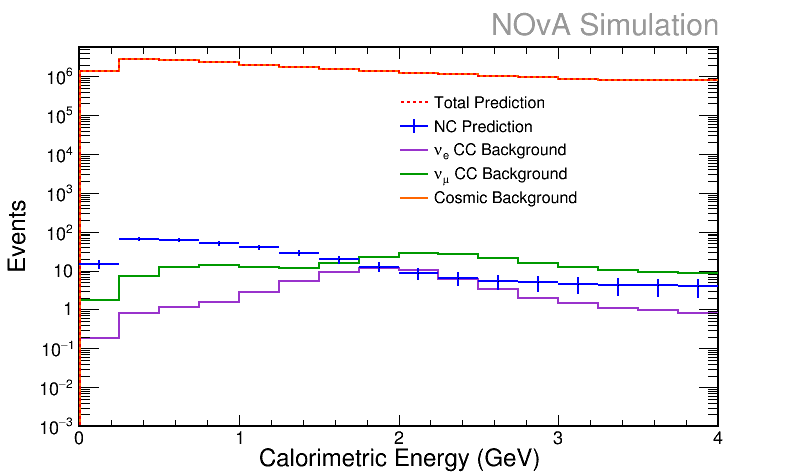
\includegraphics[width=.47\textwidth]{figures/SelE/RecoE0FD.png} &
    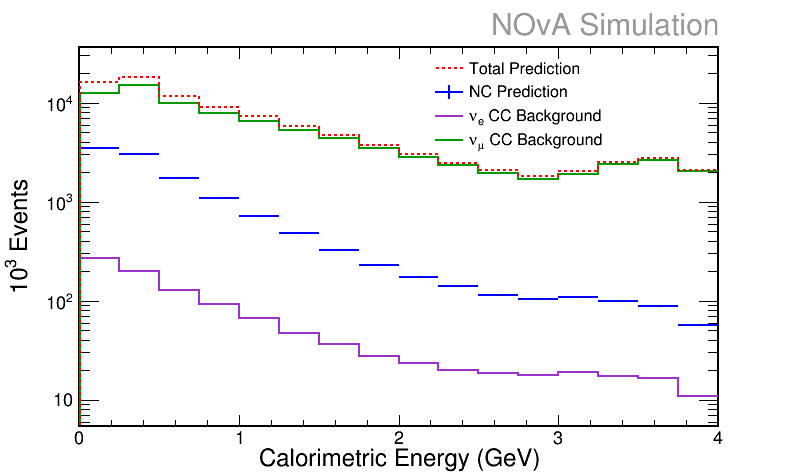
\includegraphics[width=.47\linewidth]{figures/SelE/RecoE0ND.png} \\
  \end{tabular}
  \caption[Energy Spectra After Data Quality Cuts]{Energy spectra after Data Quality cuts for the FD (left) and ND (right).}
  \label{fig:NP1DataQual}
\end{figure}

\clearpage
\section{Event Quality}
\label{sec:SelEQ}

Event quality cuts are the first applied to individual events and ensure that there is enough reconstructed information to be properly analyzed and that there were no obvious reconstruction failures. As with the data quality cuts above, these cuts were taken directly from the $\nue$ \cite{ref:EQNuEND, ref:EQNuEFD} and $\numu$ \cite{ref:EQNuMu} analyses. Two of the cuts within this suite simply require the presence of a reconstructed vertex and a shower object. These reconstructed objects are used more extensively in later stages, so the event quality cuts make sure they are available. Other quantities considered are the number of hits per plane, distance between the reconstructed vertex and leading shower, and number of contiguous planes. Events with a high number of hits per plane are cut to remove so called `FEB Flashers,' an event most often triggered by high energy cosmic rays. Likewise, events with a low number of contiguous planes are most often associated with very vertical cosmic rays. Finally, the a large distance between a vertex and leading shower is considered a reconstruction failure. These cuts are summarized with the exact parameters used for the cuts in table \ref{tab:EventQual}. The number of events before and after the event quality cuts are listed in table \ref{tab:NP1EventQual}, and figure \ref{fig:NP1EventQual} shows the energy spectra of the events that pass these cuts.
\begin{table}[p]
  \begin{center}
    \begin{tabular}{c c c}
      \hline\hline
      Event Quality Metric & Metric for Event to Pass \\
      \hline
      Number of vertex objects & $> 0$ \\
      Number of shower objects & $> 0$ \\
      Number of hits per plane & $< 8$ \\
      Number of contiguous planes & $> 2$ \\
      Distance between vertex and leading shower & $< 100\unit{cm}$ \\
      \hline
    \end{tabular}
    \caption[Event Quality Cuts]{Quality cuts applied to individual events to ensure properly reconstructed quantities.}
    \label{tab:EventQual}
  \end{center}
\end{table}

\begin{table}[p]
  \begin{center}
    \begin{tabular}{c c c c c}
      \hline\hline
      Cut Level & NC & $\numu$ CC & $\nue$ CC & Cosmic \\
      \hline
      \multicolumn{5}{l}{FD:} \\
      Data Quality & $337.0$ & $230.6$ & $58.5$ & $23.4 \times 10^{6}$ \\
      $+$Event Quality & $210.6$ & $112.0$ & $54.5$ & $0.340 \times 10^{6}$ \\
      \multicolumn{5}{l}{ND $(\times 10^{3})$:} \\
      Data Quality & $11930$ & $82594$ & $1011$ & \\
      $+$Event Quality & $7233$ & $45251$ & $592$ & \\
      \hline
    \end{tabular}
    \caption[Event Table: Event Quality Cuts]{The number of events before and after application of event quality cuts, at both detectors.}
    \label{tab:NP1EventQual}
  \end{center}
\end{table}

\begin{figure}[p]
  \centering
  \begin{tabular}{c c}
    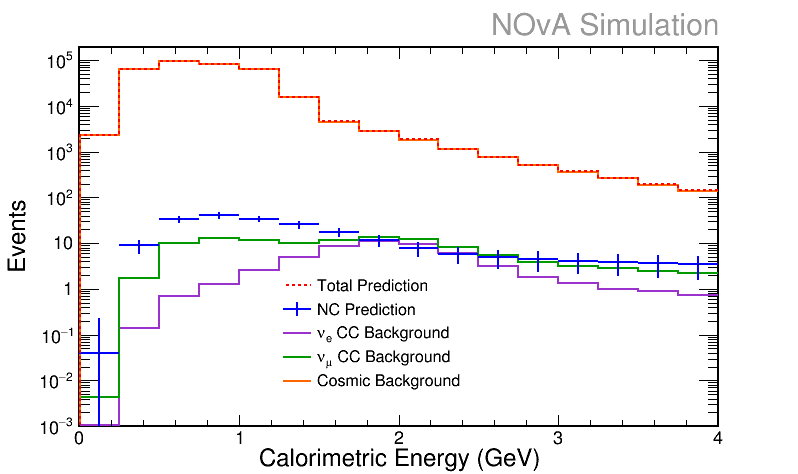
\includegraphics[width=.47\textwidth]{figures/SelE/RecoE1FD.png} &
    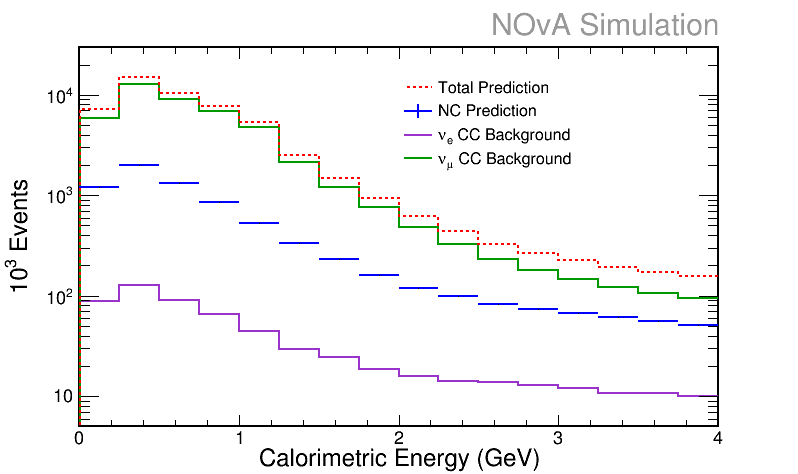
\includegraphics[width=.47\linewidth]{figures/SelE/RecoE1ND.png} \\
  \end{tabular}
  \caption[Energy Spectra After Event Quality Cuts]{Energy spectra after Event Quality cuts for the FD (left) and ND (right).}
  \label{fig:NP1EventQual}
\end{figure}

It was discovered after these cuts were frozen that the requirement for the presence of at least one shower object implicitly imposed several other cuts. These cuts are thus already applied in the spectra shown in figure \ref{fig:NP1EventQual}, but they are listed separately in table \ref{tab:NuePresel}. Since the number of hits cut was not the same at both detectors, an explicit cut is made later in the cut flow as discussed in section \ref{sec:SelNCSel}.
\begin{table}[p]
  \begin{center}
    \begin{tabular}{c c c}
      \hline\hline
      Event Quality Metric & Metric for Event to Pass & Detector \\
      \hline
      Number of hits & $> 20$ & FD \\
      Number of hits & $< 200$ & FD \\
      Number of hits & $> 10$ & ND \\
      Length of Longest Prong & $< 500\unit{cm}$ & ND, FD \\
      \hline
    \end{tabular}
    \caption[Implicit Event Quality Cuts]{Event quality cuts applied implicitly due to the requirement of at least one shower object.}
    \label{tab:NuePresel}
  \end{center}
\end{table}

\section{Fiducial Volume and Containment}
\label{sec:SelFidCont}

Fiducial volume and containment cuts are applied to remove events originating outside of the detector and to ensure that events originating inside of the detector do not have activity that escapes the detector. The fiducial volume cut is a cut on the location of the reconstructed neutrino vertex. The containment cut considers the leading prong of an event and cuts the event if the start or stop point is too close to a detector wall. The specific cuts were set separately at each detector.

\subsection{Far Detector}
\label{sec:SelFidContFD}

For the FD, the fiducial and containment cuts have the largest effect on the cosmic background. Since cosmic ray events originate above the detector, there are many more cosmic events with reconstructed vertices in the upper portion of the detector. The fiducial volume cut in Y is thus applied in an asymmetric way to eliminate more of the cosmic background. The fiducial volume cut on Z (the beam direction) is also asymmetric to account for cosmic rays entering the back of the detector hall where there is a smaller amount of rock overburden to shield these events. The fiducial volume cut on X is also applied slightly asymmetrically for a slight performance gain. Events that pass these fiducial cuts must still pass the containment cuts. For the FD, the leading prong must neither start nor stop within $10\unit{cm}$ of any detector face. Figure \ref{fig:FidCont} shows the distributions of these variables before application of the fiducial or containment cuts. Table \ref{tab:NP1FidContFD} summarizes the event rates before and after applying fiducial and containment cuts; figure \ref{fig:NP1FidContFD} show the energy spectra of events that pass these cuts.
\begin{figure}[htb]
  \centering
  \begin{tabular}{c c}
    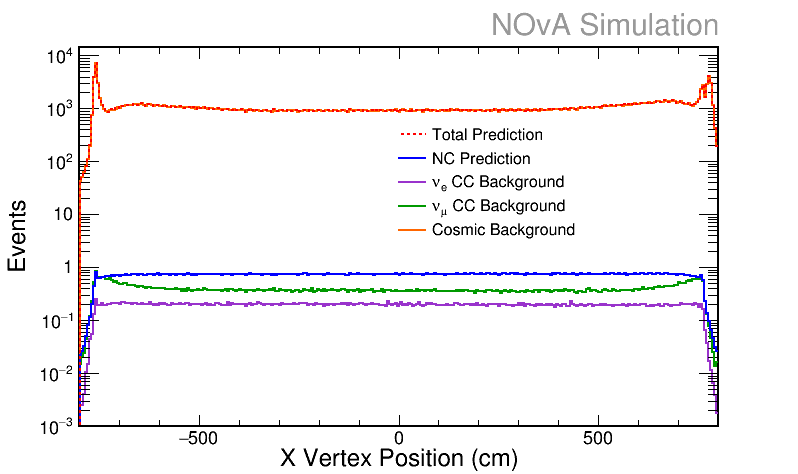
\includegraphics[width=.47\textwidth]{figures/SelNP1/NP1VtxX.png} &
    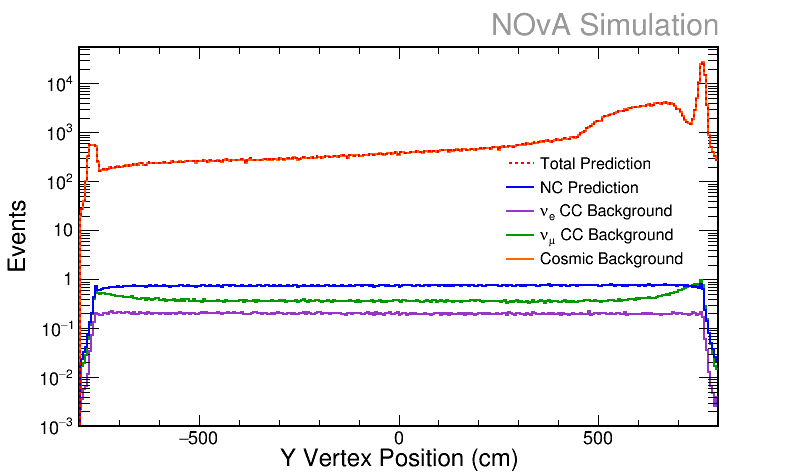
\includegraphics[width=.47\textwidth]{figures/SelNP1/NP1VtxY.png} \\
    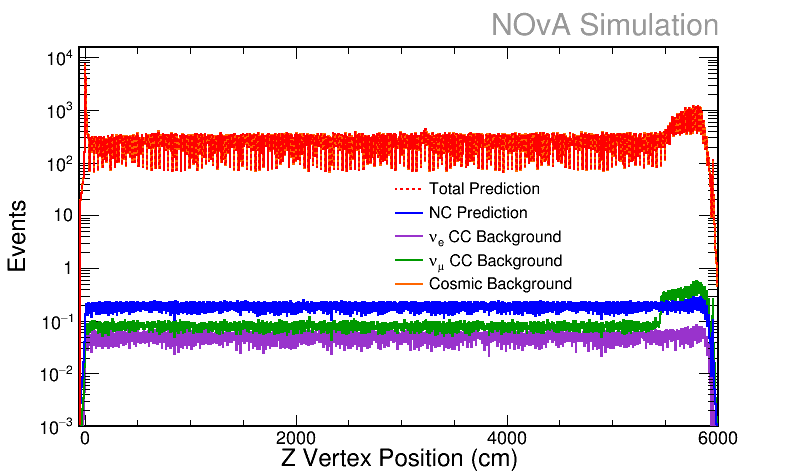
\includegraphics[width=.47\textwidth]{figures/SelNP1/NP1VtxZ.png} &
    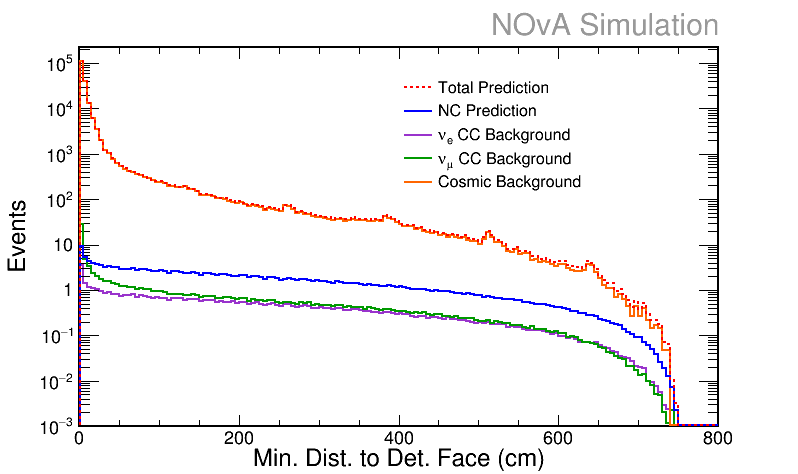
\includegraphics[width=.47\textwidth]{figures/SelNP1/NP1Cont.png} \\
  \end{tabular}
  \caption[Fiducial and Containment Variable Distributions]{Distributions of variables used for fiducial and containment cuts at the FD. The top left, top right, and bottom left show the distributions of the reconstructed vertex. The bottom right shows the minimum distance between the start or stop of the leading prong to any detector face.}
  \label{fig:FidCont}
\end{figure}

\begin{table}[htb]
  \begin{center}
    \begin{tabular}{c c c}
      \hline\hline
      Reconstructed Quantity & Metric for Event to Pass \\
      \hline
      Reconstructed Vertex X Coordinate & $-680\unit{cm} \leq vtxX \leq 650\unit{cm} $ \\
      Reconstructed Vertex Y Coordinate & $-720\unit{cm} \leq vtxY \leq 500\unit{cm}$ \\
      Reconstructed Vertex Z Coordinate & $50\unit{cm} \leq vtxZ \leq 5450\unit{cm}$ \\
      Leading prong start/stop distance to detector face & $> 10\unit{cm}$ \\
      \hline
    \end{tabular}
    \caption[FD Fiducial and Containment Cuts]{Fiducial and containment cuts applied to events in the FD.}
    \label{tab:FidContFD}
  \end{center}
\end{table}

\begin{table}[htb]
  \begin{center}
    \begin{tabular}{c c c c c}
      \hline\hline
      Cut Level & NC & $\numu$ CC & $\nue$ CC & Cosmic \\
      \hline
      ...Event Quality & $210.6$ & $112.0$ & $54.5$ & $339600$ \\
      $+$ Fiducial & $132.0$ & $46.7$ & $34.0$ & $26210$ \\
      $+$ Containment & $129.6$ & $42.7$ & $33.3$ & $4324$ \\
      \hline
    \end{tabular}
    \caption[Event Table: Fiducial and Containment Cuts, FD]{The number of events before and after application of fiducial and containment cuts at the FD.}
    \label{tab:NP1FidContFD}
  \end{center}
\end{table}

\begin{figure}[htb]
  \centering
  \begin{tabular}{c c}
    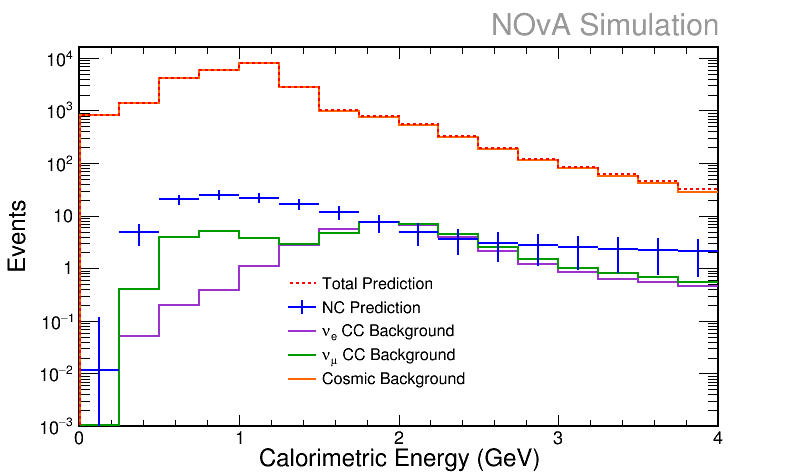
\includegraphics[width=.47\textwidth]{figures/SelE/RecoE2FD.png} &
    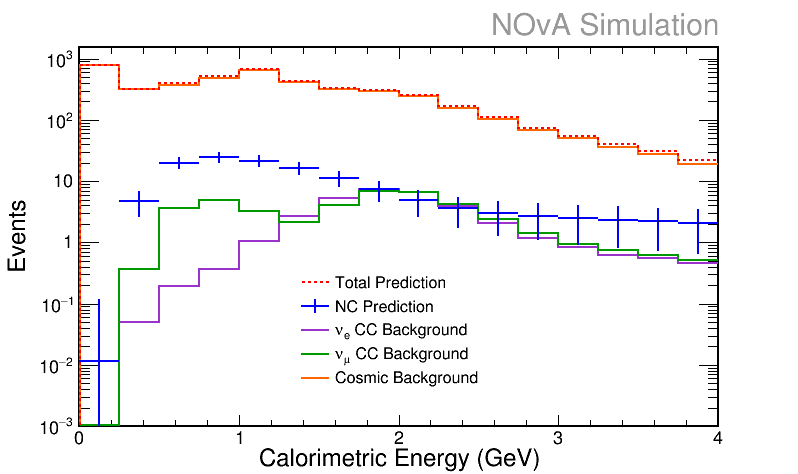
\includegraphics[width=.47\linewidth]{figures/SelE/RecoE3FD.png} \\
  \end{tabular}
  \caption[Energy Spectra After Fiducial and Containment Cuts, FD]{Energy spectra after fiducial and containment cuts for the FD. On the left, the cuts applied are data quality, event quality, and fiducial. The right plot also includes the containment cut.}
  \label{fig:NP1FidContFD}
\end{figure}

\subsection{Near Detector}
\label{sec:SelFidContND}

While the ND does not have a large cosmic background to eliminate, there are many events that originate in the rock outside of the detector that can leak into the detector. Furthermore, the small size of the ND means that many events have activity that escapes outside of the detector. The fiducial and containment cuts at the ND are designed to combat both of these effects. The fiducial cuts on the X and Y coordinates of the reconstructed vertex were applied symmetrically, with a modestly large cut to remove events that originate in the rock outside the detector. The vertex cut on Z also cuts a large portion of the detector to cut rock events that leak into the front of the detector. The containment cuts at the ND are more strict than the FD. The leading prong is required to be greater than $25\unit{cm}$ from each detector face, and every track in the event is also subject to this cut. For the cut on each track, the back `face' of the detector is considered to be the last plane of the fully active portion of the detector, effectively cutting events with activity in the muon catcher. All of these cuts are summarized in table \ref{tab:FidContND}, table \ref{tab:NP1FidContND} lists the event rates before and after the cuts are applied, and figure \ref{fig:NP1FidContND} shows the energy spectra of events that pass these cuts.
\begin{table}[htb]
  \begin{center}
    \begin{tabular}{c c c}
      \hline\hline
      Reconstructed Quantity & Metric for Event to Pass \\
      \hline
      Reconstructed Vertex X Coordinate & $-100\unit{cm} \leq vtxX \leq 100\unit{cm} $ \\
      Reconstructed Vertex Y Coordinate & $-100\unit{cm} \leq vtxY \leq 100\unit{cm}$ \\
      Reconstructed Vertex Z Coordinate & $200\unit{cm} \leq vtxZ \leq 1000\unit{cm}$ \\
      Leading prong start/stop point, distance to detector face & $> 25\unit{cm}$ \\
      Each track start/stop point, distance to detector face & $> 25\unit{cm}$ \\
      \hline
    \end{tabular}
    \caption[ND Fiducial and Containment Cuts]{Fiducial and containment cuts applied to events in the ND.}
    \label{tab:FidContND}
  \end{center}
\end{table}

\begin{table}[htb]
  \begin{center}
    \begin{tabular}{c c c c}
      \hline\hline
      Cut Level & NC & $\numu$ CC & $\nue$ CC \\
      \hline
      ...Event Quality & $7233$ & $45251$ & $592$ \\
      $+$ Fiducial & $570.7$ & $1397.8$ & $21.7$ \\
      $+$ Containment & $328.0$ & $379.4$ & $11.0$ \\
      \hline
    \end{tabular}
    \caption[Event Table: Fiducial and Containment Cuts, ND]{The number of events before and after application of fiducial and containment cuts at the ND. Here, containment refers to cuts on the distance of the leading prong and each track to the closest detector face. All numbers in this table are $\times 10^{3}$.}
    \label{tab:NP1FidContND}
  \end{center}
\end{table}

\begin{figure}[htb]
  \centering
  \begin{tabular}{c c}
    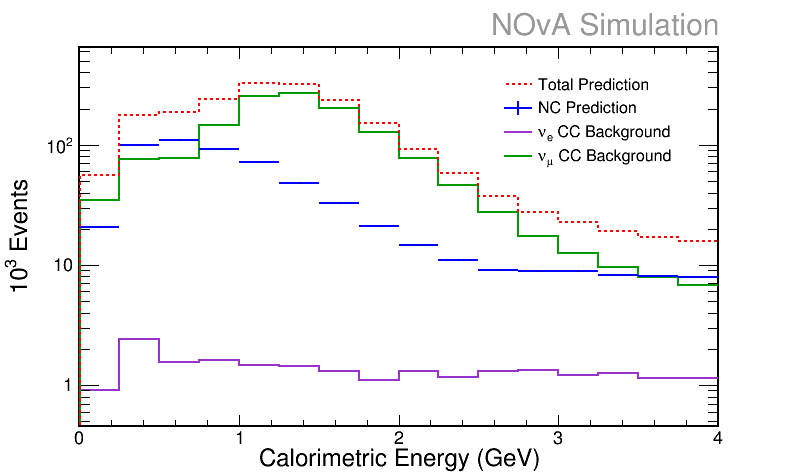
\includegraphics[width=.47\textwidth]{figures/SelE/RecoE2ND.png} &
    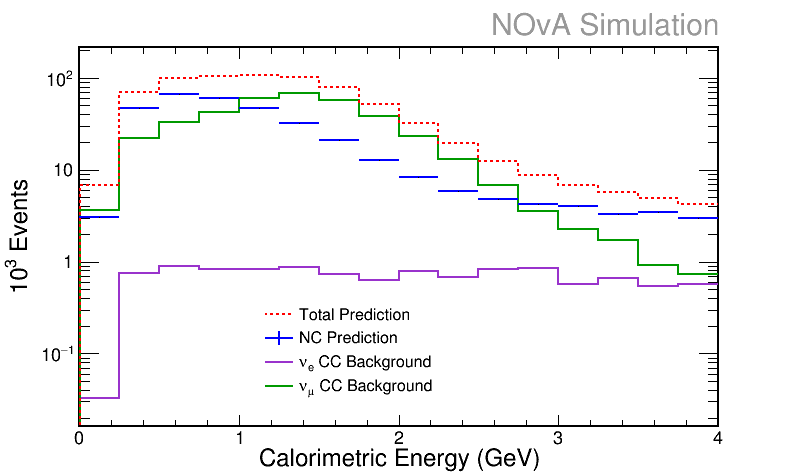
\includegraphics[width=.47\linewidth]{figures/SelE/RecoE3ND.png} \\
  \end{tabular}
  \caption[Energy Spectra After Fiducial and Containment Cuts, ND]{Energy spectra after fiducial and containment cuts for the ND. On the left, the cuts applied are data quality, event quality, and fiducial. The right plot also includes the containment cuts.}
  \label{fig:NP1FidContND}
\end{figure}

\section{NC Selection}
\label{sec:SelNCSel}

All of the cuts discussed to this point ensure that the remaining sample of events are well reconstructed, contained events. These events should all be representative of their respective types, i.e., NC, $\nue$ CC, and $\numu$ CC. The NC selection cuts are designed to select a largely pure sample of NC events from amongst the CC backgrounds. The CVN, LEM, LID, and ReMID PID distributions all have power to complete this goal. Studies showed that CVN was sufficient on its own and that combining it with the other PIDs did not improve results.

A cut on the optimized NC classifier score is the main piece of the NC selection. However, due to the implicit cuts on the number of hits discussed in section \ref{sec:SelEQ}, an explicit cut on the number of hits at both detectors is made here as well. The distributions of CVN and the number of hits at the FD are shown in figure \ref{fig:NCSel}. The cut on CVN was chosen by eye and set to keep events above $0.2$. Table \ref{tab:NCSel} summarizes the cuts used, table \ref{tab:NP1NCSel} lists the event rates before and after the selection cuts are applied, and figure \ref{fig:NP1NCSel} shows the energy distributions of events that pass these cuts.
\begin{figure}[htb]
  \centering
  \begin{tabular}{c c}
    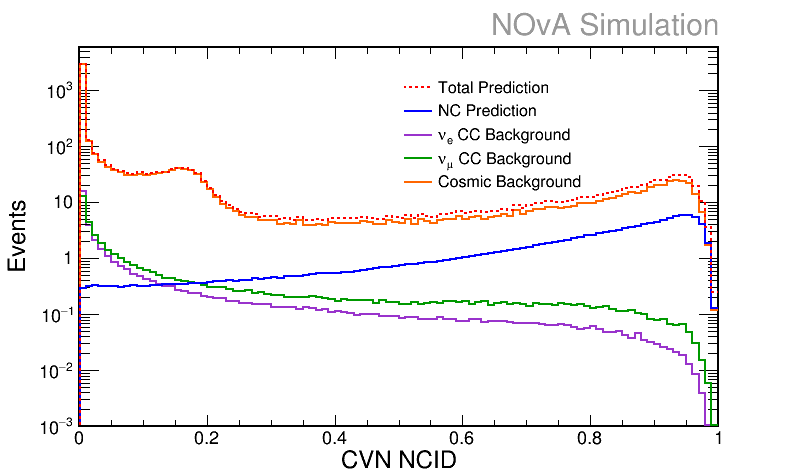
\includegraphics[width=.47\textwidth]{figures/SelNP1/NP1CVNC.png} &
    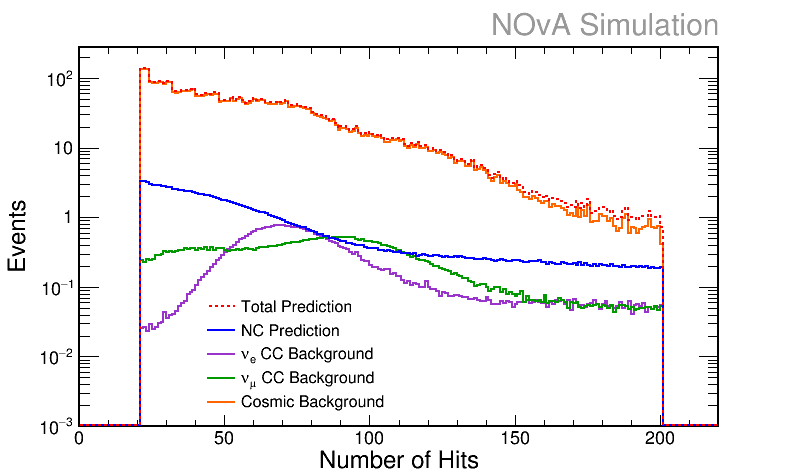
\includegraphics[width=.47\textwidth]{figures/SelNP1/NP1NHit.png} \\
  \end{tabular}
  \caption[NC Selection Variable Distributions]{Distributions of variables used for NC selection at the FD.}
  \label{fig:NCSel}
\end{figure}

\begin{table}[htb]
  \begin{center}
    \begin{tabular}{c c c}
      \hline\hline
      Selection Parameter & Metric for Event to Pass \\
      \hline
      CVN NC distribution score & $\geq 0.2$ \\
      Number of Hits & $\geq 20$, $< 200$ \\
      \hline
    \end{tabular}
    \caption[NC Selection Cuts]{NC selection cuts to reject CC events, leaving a relatively pure sample of NC events.}
    \label{tab:NCSel}
  \end{center}
\end{table}

\begin{table}[htb]
  \begin{center}
    \begin{tabular}{c c c c c}
      \hline\hline
      Cut Level & NC & $\numu$ CC & $\nue$ CC & Cosmic \\
      \hline
      \multicolumn{5}{l}{FD:} \\
      ...Containment & $129.6$ & $42.7$ & $33.3$ & $4324$ \\
      $+$NC Selection & $123.4$ & $11.5$ & $6.0$ & $643.8$ \\
      \multicolumn{5}{l}{ND $(\times 10^{3})$:} \\
      ...Containment & $328.0$ & $379.4$ & $11.0$ & \\
      $+$NC Selection & $263.9$ & $124.4$ & $3.5$ & \\
      \hline
    \end{tabular}
    \caption[Event Table: NC Selection Cuts]{The number of events before and after application of NC selection cuts, at both detectors.}
    \label{tab:NP1NCSel}
  \end{center}
\end{table}

\begin{figure}[htb]
  \centering
  \begin{tabular}{c c}
    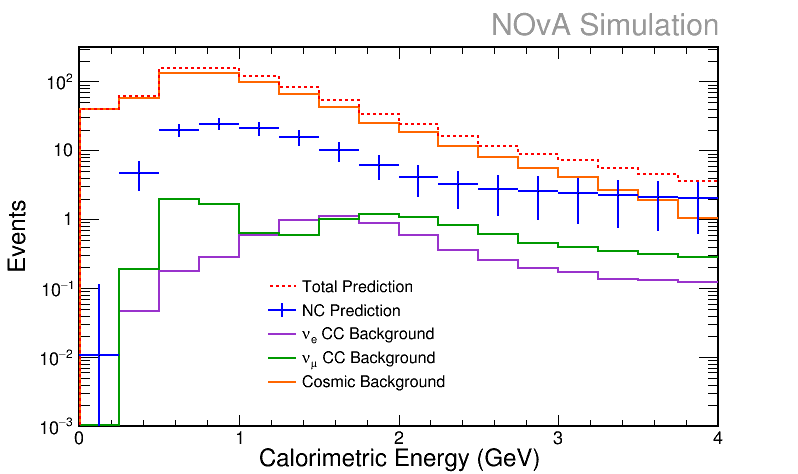
\includegraphics[width=.47\textwidth]{figures/SelE/RecoE4FD.png} &
    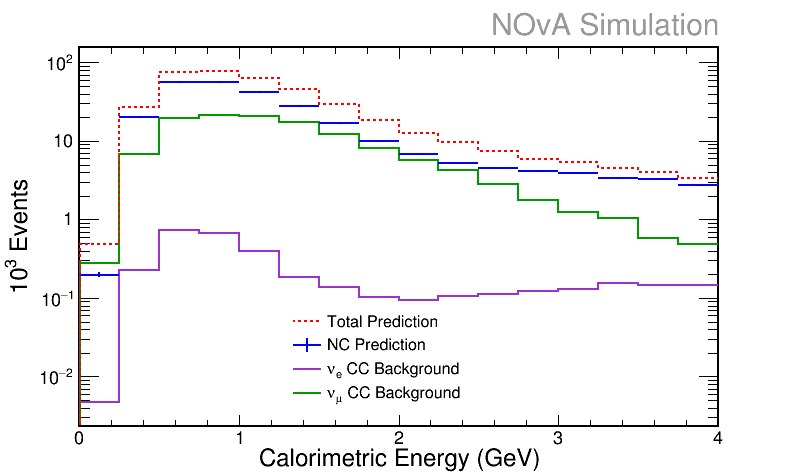
\includegraphics[width=.47\linewidth]{figures/SelE/RecoE4ND.png} \\
  \end{tabular}
  \caption[Energy Spectra After NC Selection Cuts]{Energy spectra after NC selection cuts for the FD (left) and ND (right).}
  \label{fig:NP1NCSel}
\end{figure}

Chronologically, CVN was developed later than the other PIDs and the analysis was originally developed using LID and ReMID. While they were ultimately replaced by CVN as the sole PID used in the analysis, they nevertheless provided a valuable check that CVN was behaving sensibly. The PID distributions for ReMID and LID were studied after applying the full cut flow to ensure that it was removing largely the same events, and if there were any other minor performance increases to be gained. Figure \ref{fig:NM1NCSel} shows these distributions. Based on the results, it was decided that CVN provided all of the necessary separation power and so RemID and LID were not used in the analysis.
\begin{figure}[htb]
  \centering
  \begin{tabular}{c c}
    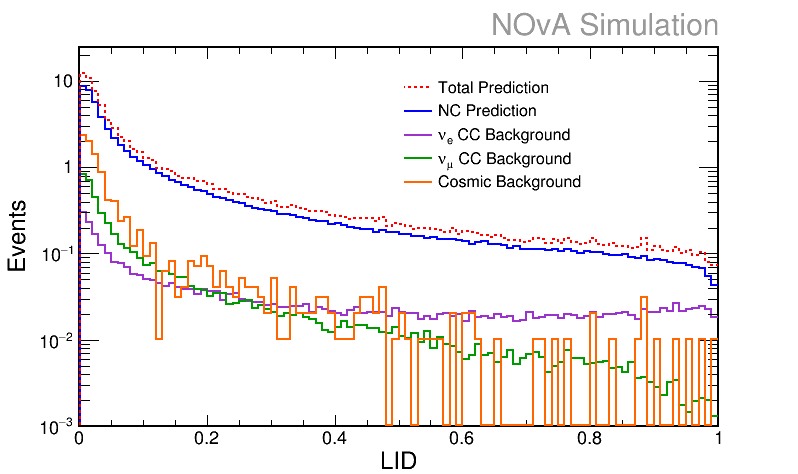
\includegraphics[width=.47\textwidth]{figures/SelNP1/NM1ELID.png} &
    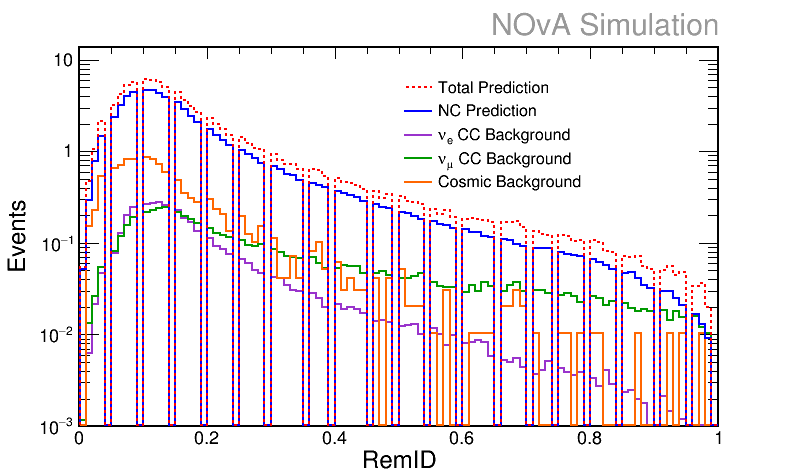
\includegraphics[width=.47\textwidth]{figures/SelNP1/NM1RmID.png} \\
  \end{tabular}
  \caption[LID and RemID Distributions at the FD]{LID and RemID distributions at the FD after all other cuts applied.}
  \label{fig:NM1NCSel}
\end{figure}

\section{Cosmic Rejection}

The final set of cuts applied to the events is cosmic rejection. While there are essentially no cosmic events at the ND, the cuts are still applied at the ND when possible to maintain similar spectra at both detectors. The main variable to discriminate against cosmics is the output of the BDT described in section \ref{sec:PIDcos}. Another powerful discriminant is the fraction of total transverse energy deposition versus total event energy deposition, originally developed for the $\nue$ appearance analysis \cite{ref:EQNuEFD}. The other cuts used for cosmic rejection are a cut on low average energy per hit, a harsher cut on the start/stop distance of the leading prong to the top of the detector, and removing events where the leading shower has a greatest likelihood of being a muon. The distributions of these variables at the FD are shown in figure \ref{fig:CosRej} and table \ref{tab:CosRej} summarizes the cosmic rejection with the values used for the actual cuts. Table \ref{tab:NP1CosRej} lists the event rates before and after the cosmic rejection cuts are applied, and figure \ref{fig:Sel} shows the energy distributions of events that pass these cuts.
\begin{figure}[htb]
  \centering
  \begin{tabular}{c c}
    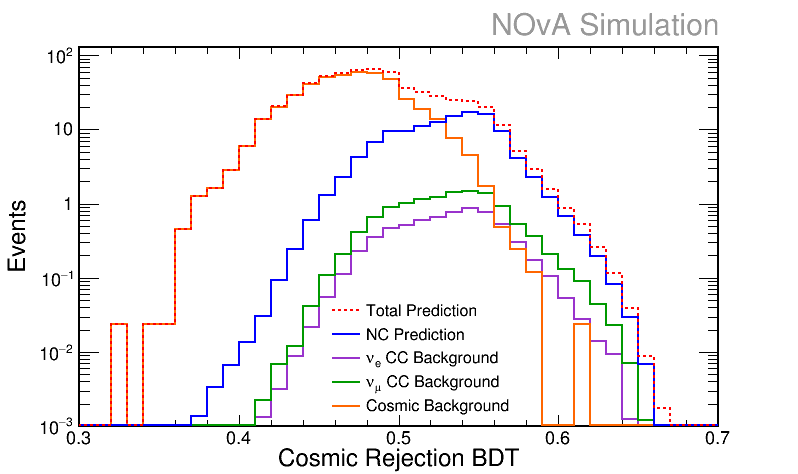
\includegraphics[width=.47\textwidth]{figures/SelNP1/NP1NmCP.png} &
    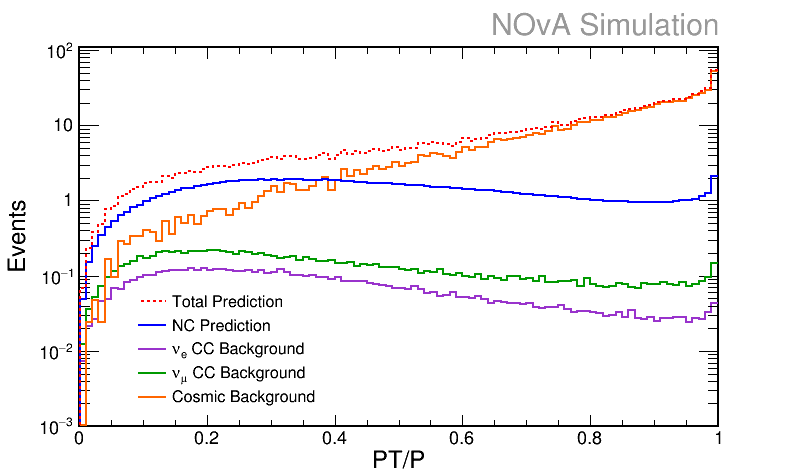
\includegraphics[width=.47\textwidth]{figures/SelNP1/NP1PPTP.png} \\
    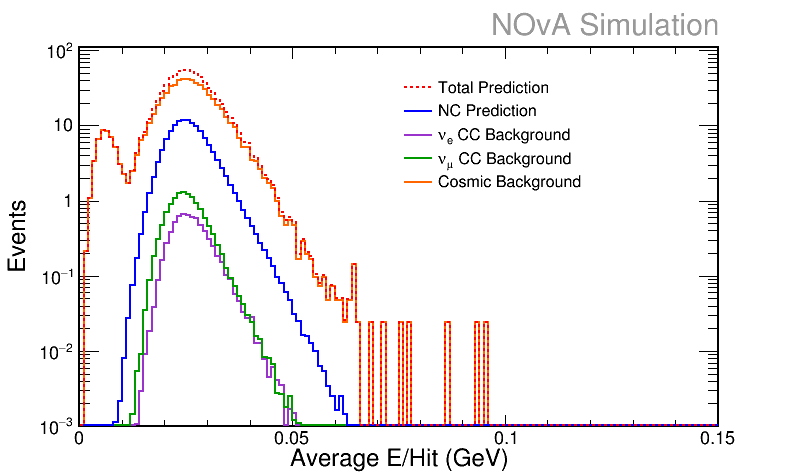
\includegraphics[width=.47\textwidth]{figures/SelNP1/NP1EHit.png} &
    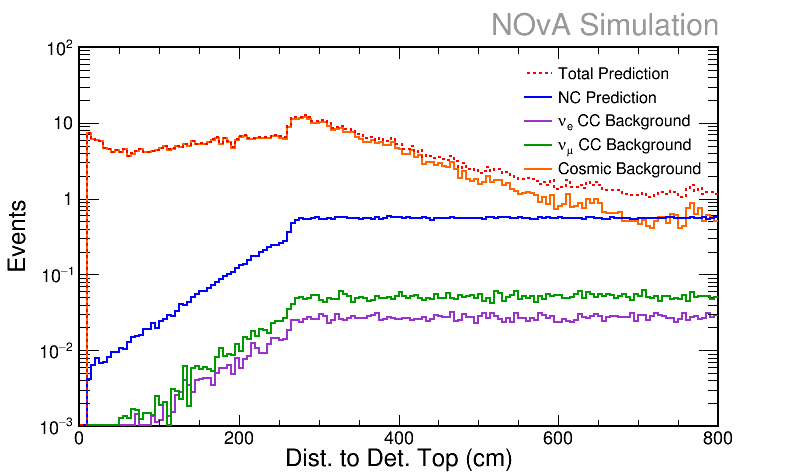
\includegraphics[width=.47\textwidth]{figures/SelNP1/NP1DistTop.png} \\
    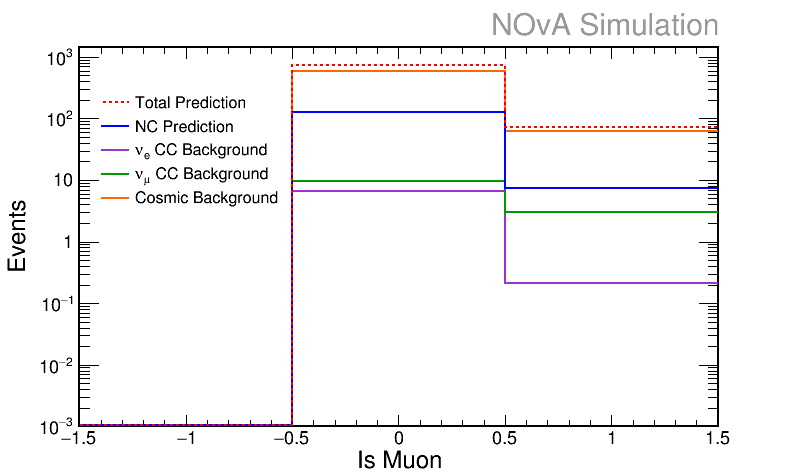
\includegraphics[width=.47\textwidth]{figures/SelNP1/NP1IsMu.png} & \\
  \end{tabular}
  \caption[Cosmic Rejection Variable Distributions]{Distributions of variables used for cosmic rejection at the FD.}
  \label{fig:CosRej}
\end{figure}

\begin{table}[htb]
  \begin{center}
    \begin{tabular}{c c}
      \hline\hline
      Selection Parameter & Metric for Event to Pass \\
      \hline
      Cosmic BDT Score & $> 0.5$ (FD Only) \\
      Particle Transverse Momentum Fraction & $< 0.8$ \\
      LID Algorithm $\mu$ Identifier & False \\
      Average Energy per Hit & $> 18\unit{MeV}$ (FD), $> 9\unit{MeV}$ (ND) \\
      Distance of Leading Prong to Detector Top & $\geq 480\unit{cm}$ (FD Only) \\
      Calorimetric Energy & $> 0.5\unit{GeV}$, $< 4.0\unit{GeV}$ \\
      \hline
    \end{tabular}
    \caption[Final Selection Cuts]{Final selection cuts applied to all events.}
    \label{tab:CosRej}
  \end{center}
\end{table}

\begin{table}[htb]
  \begin{center}
    \begin{tabular}{c c c c c}
      \hline\hline
      Cut Level & NC & $\numu$ CC & $\nue$ CC & Cosmic \\
      \hline
      \multicolumn{5}{l}{FD:} \\
      ...NC Selection & $123.4$ & $11.5$ & $6.0$ & $643.8$ \\
      $+$ Cosmic Rejection & $65.0$ & $5.0$ & $3.7$ & $11.0$ \\
      \multicolumn{5}{l}{ND $(\times 10^{3})$:} \\
      ...NC Selection & $263.9$ & $124.4$ & $3.5$ \\
      $+$ Cosmic Rejection & $198.3$ & $77.5$ & $2.6$ \\
      \hline
      \hline
    \end{tabular}
    \caption[Event Table: FD Cosmic Rejection Cuts]{The number of events after each cut level at the FD.}
    \label{tab:NP1CosRej}
  \end{center}
\end{table}

\begin{figure}[htb]
  \centering
  \begin{tabular}{c c}
    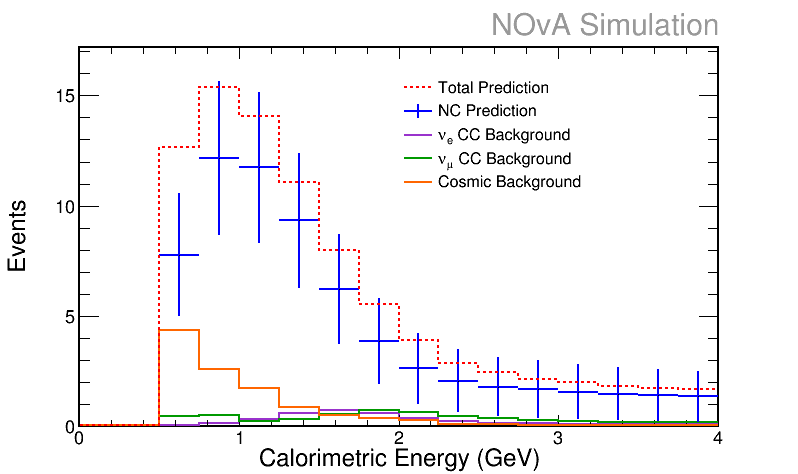
\includegraphics[width=.47\textwidth]{figures/SelE/RecoE5FD.png} &
    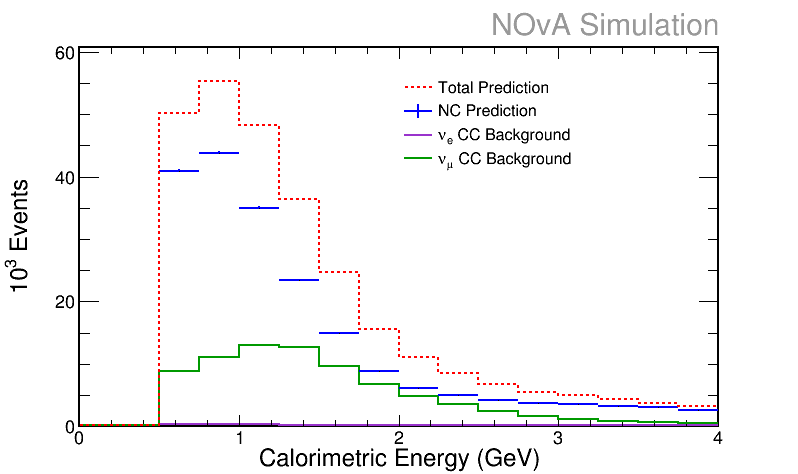
\includegraphics[width=.47\textwidth]{figures/SelE/RecoE5ND.png} \\
  \end{tabular}
  \caption[Energy Spectra After All Cuts]{Energy spectra after all cuts for the FD (left) and ND (right).}
  \label{fig:Sel}
\end{figure}

\section{Summary}

The final selection combines all of the previous sections with explicit energy cuts applied at both low and high energy. A low energy cut rejecting events below $0.5\unit{GeV}$ was used to reject very low energy events that could be subject to threshold events, and a high energy cut rejecting events above $4\unit{GeV}$ was placed due to diverging ND and FD selection efficiencies above that point. These energy cuts are listed in table \ref{tab:NP1CosRej}. The event rates at each level of cut are summarized for the FD in table \ref{tab:FDSel}, and in table \ref{tab:NDSel} for the ND. The final energy spectra are shown in figure \ref{fig:Sel}.
\begin{table}[htb]
  \begin{center}
    \begin{tabular}{c c c c c}
      \hline\hline
      Cut Level & NC & $\numu$ CC & $\nue$ CC & Cosmic \\
      \hline
      Data Quality & $337.0$ & $230.6$ & $58.5$ & $23.42 \times 10^{6}$ \\
      $+$ Event Quality & $210.6$ & $112.0$ & $54.5$ & $339600$ \\
      $+$ Fiducial & $132.0$ & $46.7$ & $34.0$ & $26210$ \\
      $+$ Containment & $129.6$ & $42.7$ & $33.3$ & $4324$ \\
      $+$ NC Selection & $123.4$ & $11.5$ & $6.0$ & $643.8$ \\
      $+$ Cosmic Rejection & $65.0$ & $5.0$ & $3.7$ & $11.0$ \\
      \hline
    \end{tabular}
    \caption[Event Table: FD Selection Cuts]{The number of events after each cut level at the FD.}
    \label{tab:FDSel}
  \end{center}
\end{table}

\begin{table}[htb]
  \begin{center}
    \begin{tabular}{c c c c}
      \hline\hline
      Cut Level & NC & $\numu$ CC & $\nue$ CC \\
      \hline
      Data Quality & $11930$ & $82594$ & $1011$ \\
      $+$Event Quality & $7233$ & $45251$ & $592$ \\
      $+$ Fiducial & $570.7$ & $1397.8$ & $21.7$ \\
      $+$ Containment & $328.0$ & $379.4$ & $11.0$ \\
      $+$ NC Selection & $263.9$ & $124.4$ & $3.5$ \\
      $+$ Cosmic Rejection & $198.3$ & $77.5$ & $2.6$ \\
      \hline
    \end{tabular}
    \caption[Event Table: ND Selection Cuts]{The number of events after each cut level at the ND. All numbers in this table are $\times 10^{3}$.}
    \label{tab:NDSel}
  \end{center}
\end{table}